\documentclass[a4paper,12pt]{report}
\usepackage[T2A]{fontenc}
\usepackage[utf8]{inputenc}
\usepackage[english,russian]{babel}
\usepackage{graphicx}
\usepackage{wrapfig}
\usepackage{mathtext} 				% русские буквы в фомулах
\usepackage{amsmath,amsfonts,amssymb,amsthm,mathtools} % AMS
\usepackage{icomma} % "Умная" запятая: $0,2$ --- число, $0, 2$ --- перечисление
\usepackage{capt-of}
\usepackage{appendix}
\usepackage{multirow}
\usepackage{hyperref}
\usepackage{floatrow}
\usepackage[left=2cm,right=2cm,
    top=2cm,bottom=2cm,bindingoffset=0cm]{geometry}
\usepackage{multicol} % Несколько колонок
\usepackage{gensymb}
\title{Отчёт по лабораторной работе № 5.2.2 и № 5.2.3. 

Изучение спектров атома водорода и молекулы йода.}
\author{Плюскова Н.А. Б04-004 }
\date{\today}
\begin{document}
\maketitle
\section*{1. Аннотация}
В работе будут исследованы сериальные закономерности в оптическом спектре водорода и спектр поглощения паров йода в видимой области.
	
С помощью информации о спектральных линиях неона и ртути будет проградуирован спектрометр и построен соответствующий график.
	
Мы получим длины волн линий $H_{\alpha}$, $H_{\beta}$,$H_{\gamma}$ и  $H_{\delta}$ серии Бальмера, вычислим постоянную Ридберга.

Получим длины волн, соответствующие некоторым электронно-колебательным переходам из основного состояния в возбуждённое. Вычислим энергию колебательного кванта возбуждённого состояния молекулы, энергию электронного перехода и энергию диссоциации молекулы в основном и в возбуждённом состояниях.

\section*{2. Теоретические сведения}
Длины волн спектральных линий водородоподобного атома описываются формулой
\begin{equation}
    \frac{1}{\lambda_m_n} = RZ^2(\frac{1}{n^2} - \frac{1}{m^2}),
\end{equation}
где $R$ - постоянная Ридберга, а $m, n$ -  целые числа. \par
Использование постулатов Бора с учётом кулоновского взаимодействия между ядром и электроном позволяет легко определить возможные энергетические состояния водородоподобного атома. Если считать ядро неподвижным, то эти энергетические состояния определяются выражением
\begin{equation}
    E_n = -\frac{2 \pi^2 m_e e^4 Z^2}{h^2} \frac{1}{n^2}
\end{equation}

\begin{figure}[h]
    \centering
    \includegraphics[width=6cm]{fig3.PNG}
    \caption{Уровни энергии атома водорода и образование спектральных серий}
    \label{fig:vac}
\end{figure}

Знание энергетических состояний атома позволяет в соответствии с формулой (2) определить возможные частоты его излучения и объяснить наблюдаемые закономерности. \par
В данной работе изучается серия Бальмера, линии которой лежат в видимой области, и изотопический сдвиг между линиями водорода. Для серии Бальмера в формуле (1) $n = 2$. Величина $m$ для первых четырёх линий этой серии принимает значение 3, 4, 5, 6. \par
Боровский радиус (радиус первой орбиты) для электрона в поле ядра с зарядом $Z$:
\begin{equation}
    r_B = \frac{\hbar^2}{Z m_e e^2}
\end{equation}
Энергия основного состояния:
\begin{equation}
    E = -\frac{m_e e^4}{2 \hbar^2}Z^2 = -R Z^2
\end{equation}
Аналогичным образом могут быть найдены энергии возбуждённых состояний. Дискретные значения энергии электрона в атоме получаются из того условия, что на длине орбиты, по которой движется электрон, должно укладываться целое число волн де Бройля. Если радиус орбиты равен $r$, то $n$-му состоянию электрона соответствует условие 
\begin{equation}
    2 \pi r = \lambda n (n \in \mathbb{N}) ; m_e v_n = \frac{nh}{2 \pi r}
\end{equation}

Аналогично пп. (3)-(4):
\begin{equation}
     r_B = \frac{n^2 \hbar^2}{Z m_e e^2}
\end{equation}

\begin{equation}
    E = -\frac{m_e e^4}{2 \hbar^2} \frac{1}{n^2} Z^2 = -R \frac{Z^2}{n^2}
\end{equation}

\section*{3. Экспериментальная установка}
Для измерения длин волн спектральных линий в работе используется стеклянно-призменный монохроматор-спектрометр УМ-2, предназначенный для спектральных исследований в диапазоне от 0,38 до 1 мкм

\begin{figure}[h]
    \centering
    \includegraphics[width=10cm]{fig2.PNG}
    \caption{Устройство монохроматора УМ-12}
    \label{fig:vac}
\end{figure}

Спектрометр нуждается в дополнительной градуировке, проводящейся по спектру ртутной лампы с известными длинами волн спектральных линий.

Для наблюдения спектра водорода используется установка, изображённая на Рис. 2А. Источником света для наблюдения служит водородная трубка Н-образной формы, в состав газа которой добавлены водные пары для увеличения яркости интересующих нас линий. Источник Л помещается на оптическую скамью вместе с конденсером К, так что свет концентрируется на входной щели 1. Далее через коллиматорный объектив 2 свет попадает на сложную спектральную призму, состояющую из призм П$_1$, П$_2$ и П$_3$. Первые две призмы обладают большой дисперсией, а промежуточная П$_3$ поворачивает лучи -- такое устройство позволяет складывать дисперии П$_1$ и П$_2$. После прохождения призмы свет попадает в зрительную трубу 4-5, объектив которой даёт изображение входной щели различных цветов.
\begin{figure}[h]
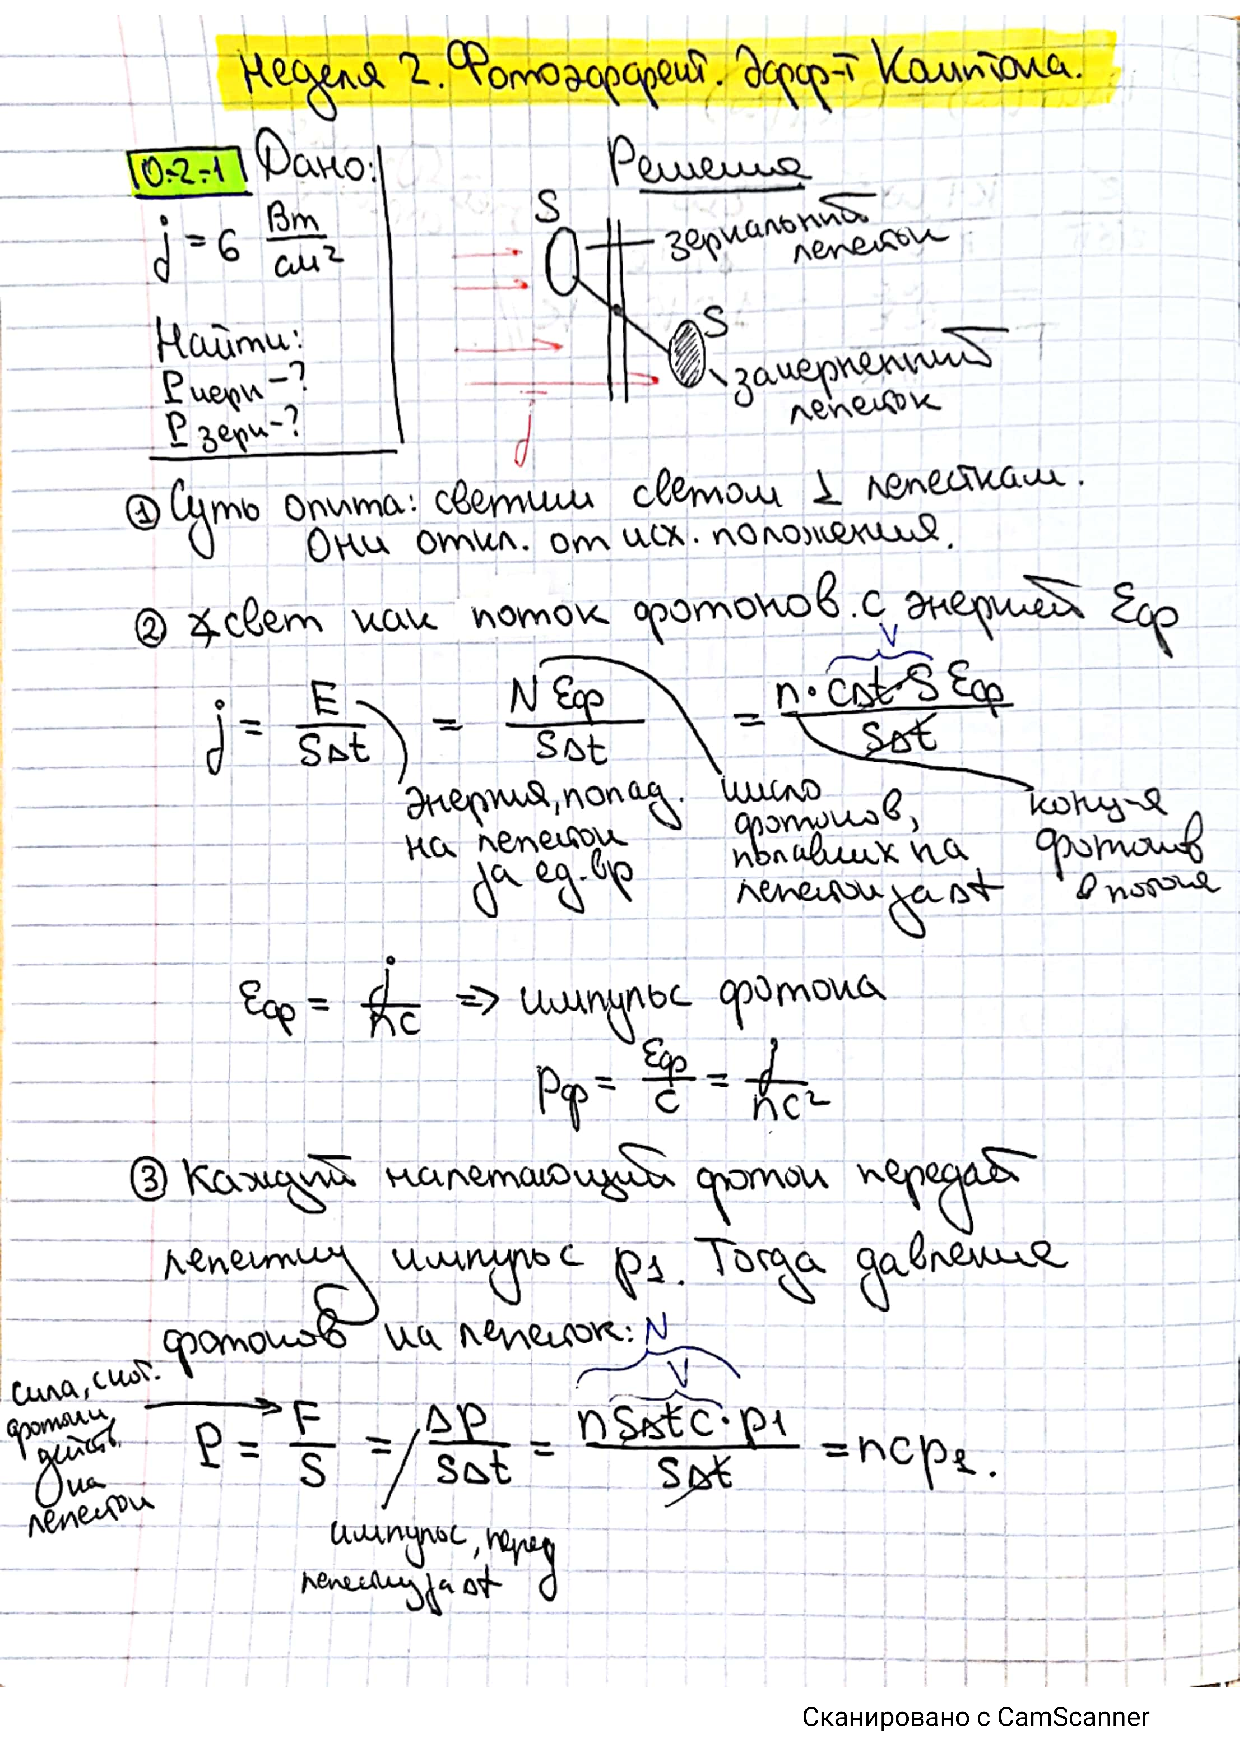
\includegraphics[scale=0.5]{2.png}
\centering
\caption{Установки для наблюдения линий А. водорода; Б. йода.}
\end{figure} 
На Рис. 2Б изображена схема установки, используемой для наблюдения спектра йода. Спектр поглощения паров йода наблюдается визуально на фоне сплошного спектра лампы накаливания 1, питаемой от блока питания 2. Кювета 3 с кристаллами йода подогревается нихромовой спиралью, подключённой вместе с лампой накаливания к блоку питания. Линза 4 используется как конденсор. В результате подогрева кристаллы йода частично возгоняются, образуя пары
с лёгкой фиолетовой окраской. Спектрометр 5 позволяет визуально наблюдать линии поглощения молекул йода на фоне сплошного спектра излучения лампы накаливания видимой области.
\section*{4. Ход работы}
Проградуируем спектрометр по спектру неона и ртути:

\begin{table}[H]
\begin{tabular}{|ccc|}
\hline
\multicolumn{3}{|c|}{Ртуть}                                                    \\ \hline
\multicolumn{1}{|c|}{$\lambda$, $A^{o}$} & \multicolumn{1}{c|}{$\theta, ^{o}$} & $\sigma_{\theta}, ^{o}$        \\ \hline
\multicolumn{1}{|c|}{6907}   & \multicolumn{1}{c|}{2919}  & \multirow{8}{*}{1} \\ \cline{1-2}
\multicolumn{1}{|c|}{6234}   & \multicolumn{1}{c|}{2687}  &                    \\ \cline{1-2}
\multicolumn{1}{|c|}{5791}   & \multicolumn{1}{c|}{2481}  &                    \\ \cline{1-2}
\multicolumn{1}{|c|}{5770}   & \multicolumn{1}{c|}{2470}  &                    \\ \cline{1-2}
\multicolumn{1}{|c|}{5461}   & \multicolumn{1}{c|}{2292}  &                    \\ \cline{1-2}
\multicolumn{1}{|c|}{4916}   & \multicolumn{1}{c|}{1868}  &                    \\ \cline{1-2}
\multicolumn{1}{|c|}{4358}   & \multicolumn{1}{c|}{1206}  &                    \\ \cline{1-2}
\multicolumn{1}{|c|}{4047}   & \multicolumn{1}{c|}{651}   &                    \\ \hline
\end{tabular}
\caption{Градуировка спектрометра по спектру ртути}
\end{table}

\begin{table}[H]
\begin{tabular}{|ccc|}
\hline
\multicolumn{3}{|c|}{Неон}                                                      \\ \hline
\multicolumn{1}{|c|}{$\lambda$, $A^{o}$} & \multicolumn{1}{c|}{$\theta, ^{o}$} & $\sigma_{\theta}, ^{o}$         \\ \hline
\multicolumn{1}{|c|}{7032}   & \multicolumn{1}{c|}{2956}  & \multirow{25}{*}{1} \\ \cline{1-2}
\multicolumn{1}{|c|}{6929}   & \multicolumn{1}{c|}{2926}  &                     \\ \cline{1-2}
\multicolumn{1}{|c|}{6717}   & \multicolumn{1}{c|}{2860}  &                     \\ \cline{1-2}
\multicolumn{1}{|c|}{6678}   & \multicolumn{1}{c|}{2848}  &                     \\ \cline{1-2}
\multicolumn{1}{|c|}{6599}   & \multicolumn{1}{c|}{2820}  &                     \\ \cline{1-2}
\multicolumn{1}{|c|}{6533}   & \multicolumn{1}{c|}{2798}  &                     \\ \cline{1-2}
\multicolumn{1}{|c|}{6507}   & \multicolumn{1}{c|}{2790}  &                     \\ \cline{1-2}
\multicolumn{1}{|c|}{6402}   & \multicolumn{1}{c|}{2752}  &                     \\ \cline{1-2}
\multicolumn{1}{|c|}{6383}   & \multicolumn{1}{c|}{2745}  &                     \\ \cline{1-2}
\multicolumn{1}{|c|}{6334}   & \multicolumn{1}{c|}{2727}  &                     \\ \cline{1-2}
\multicolumn{1}{|c|}{6305}   & \multicolumn{1}{c|}{2715}  &                     \\ \cline{1-2}
\multicolumn{1}{|c|}{6267}   & \multicolumn{1}{c|}{2699}  &                     \\ \cline{1-2}
\multicolumn{1}{|c|}{6217}   & \multicolumn{1}{c|}{2679}  &                     \\ \cline{1-2}
\multicolumn{1}{|c|}{6164}   & \multicolumn{1}{c|}{2658}  &                     \\ \cline{1-2}
\multicolumn{1}{|c|}{6143}   & \multicolumn{1}{c|}{2647}  &                     \\ \cline{1-2}
\multicolumn{1}{|c|}{6096}   & \multicolumn{1}{c|}{2630}  &                     \\ \cline{1-2}
\multicolumn{1}{|c|}{6074}   & \multicolumn{1}{c|}{2618}  &                     \\ \cline{1-2}
\multicolumn{1}{|c|}{6030}   & \multicolumn{1}{c|}{2596}  &                     \\ \cline{1-2}
\multicolumn{1}{|c|}{5976}   & \multicolumn{1}{c|}{2574}  &                     \\ \cline{1-2}
\multicolumn{1}{|c|}{5945}   & \multicolumn{1}{c|}{2560}  &                     \\ \cline{1-2}
\multicolumn{1}{|c|}{5882}   & \multicolumn{1}{c|}{2529}  &                     \\ \cline{1-2}
\multicolumn{1}{|c|}{5852}   & \multicolumn{1}{c|}{2514}  &                     \\ \cline{1-2}
\multicolumn{1}{|c|}{5401}   & \multicolumn{1}{c|}{2250}  &                     \\ \cline{1-2}
\multicolumn{1}{|c|}{5341}   & \multicolumn{1}{c|}{2210}  &                     \\ \cline{1-2}
\multicolumn{1}{|c|}{5331}   & \multicolumn{1}{c|}{2202}  &                     \\ \hline
\end{tabular}
\caption{Градуировка спектрометра по спектру неона}
\end{table}

По полученным данным построим градуировочную кривую:

	\begin{figure}[H]
		\centering
		\includegraphics[width=0.7\linewidth]{grad.png}
		\caption{Градуировочная кривая $\lambda(\theta)$}
		\label{ris mu}
	\end{figure}

Получаем нелинейную градуировку, которую аппроксимируем полиномом 5 степени:
\begin{equation*}
    y = A + Bx + Cx^2 + Dx^3 + Ex^4
\end{equation*}
\begin{center}
$A = 4228; \ B = -1,1;\ C = 1,7 * 10^{-3};\ D = -7,2 * 10^{-7}; \ E = 1,3 * 10^{-10}$    
\end{center}

Измерим положения линий $H_{\alpha},H_{\beta},H_{\gamma}, H_{\delta}$ водорода и с помощью градуировочной кривой найдем длины волн этих линий:

\begin{table}[H]
\begin{tabular}{|c|c|c|c|}
\hline
             & $\theta, ^{o}$ & $\lambda$, $A^{o}$ & $\sigma_{\lambda}$, $A^{o}$ \\ \hline
$H_{\alpha}$ & 2808  & 6684,4 & 2,9               \\ \hline
$H_{\beta}$ & 1816  & 4938,6 & 1,1               \\ \hline
$H_{\gamma}$ & 1170  & 4358,6 & 0,8               \\ \hline
$H_{\delta}$ & 762   & 4102,2 & 0,5               \\ \hline
\end{tabular}
\caption{Положение линий водорода и их длины волн}
\end{table}

Воспользуемся формулой (1), чтобы найти постоянную Ридберга для спектральных линий водорода:

\begin{equation*}
    R = \frac{1}{\lambda_{mn}Z^{2}(\frac{1}{n^{2}} - \frac{1}{m^{2}})}
\end{equation*}

\begin{table}[H]
\begin{tabular}{|c|c|c|}
\hline
             & $R$ * 10^{6}, m^{-1}     & $\sigma_{R}*10^{6}, m^{-1} $ \\ \hline
$H_{\alpha}$ & 10,84 & 0,04    \\ \hline
$H_{\beta}$ & 10,8  & 0,02    \\ \hline
$H_{\gamma}$ & 10,93 & 0,02    \\ \hline
$H_{\delta}$ & 10,97 & 0,01    \\ \hline
\end{tabular}
\end{table}

Получим $R \approx (10,89 \pm 0,04) * 10^{6} m^{-1}$, что в пределах 2$\sigma$ сходится с табличным значением $R =  10,97 * 10^{6} m^{-1}$

Погрешность измерения постоянной Ридберга считалась по формуле:
\begin{equation*}
    \sigma_{R} = \frac{\sigma_{\lambda_{mn}}}{\lambda_{mn}^{2}Z^{2}(\frac{1}{n^{2}} - \frac{1}{m^{2}})}
\end{equation*}

Для йода найдем длину волны одной из самых длинноволновых хорошо видимых линий поглощения, шестую длинноволновую линию от нее и границы схождения спектра:

\begin{table}[H]
\begin{tabular}{|c|c|c|c|c|c|}
\hline
               & $\theta, ^{o}$ & $\lambda$, $A^{o}$ & $\sigma_{\lambda}$ & $h\nu$, эВ  & $\sigma_{h\nu}$, эВ \\ \hline
$h\nu_{(1,0)}$ & 2658  & 6282,8 & 2,5               & 1,977 & 0,081     \\ \hline
$h\nu_{(1,5)}$ & 2552  & 6039,7 & 2,2               & 2,057 & 0,073     \\ \hline
$h\nu_{gr}$    & 2054  & 5215,4 & 1,3               & 2,382 & 0,068     \\ \hline
\end{tabular}
\end{table}


Вычислим энергию колебательного кванта возмущенного состояния молекулы йода по формуле:
\begin{equation*}
  h\nu_{2} = \frac{h\nu_{1,5}-h\nu_{1,0}}{5} = (0,016 \pm 0,002)\text{ эВ}
\end{equation*}

Погрешность измерения энергии колебательного кванта возмущенного состояния посчитали следующим образом:

Зная, что $h\nu_{1} = 0,027$ эВ - энергия колебательного кванта основного состояния, а $E_{A} = 0,94$ эВ - энергия возмущения атома, а также следующие соотношения:

\begin{equation*}
			\begin{cases}
				D_1+E_A=h \nu_{gr},\\
				h\nu_{gr}=D_2+h \nu_{el},\\
				h\nu_{1,0}=h \nu_{el}+h\nu_2-\dfrac{3}{2}h\nu_1,\\
					h\nu_{1,5}=h \nu_{el}+\dfrac{11}{2}h\nu_2-\dfrac{3}{2}h\nu_1.
			\end{cases}
		\end{equation*}

Найдем $h \nu_{el}$ - энергию электронного перехода,$D_{1}$ - энергию диссоциации молекулы в основном состоянии,$D_{2}$ - энергию диссоциации молекулы в возбужденном состоянии. Решая систему уравнений, получим:
\[\boxed{\nu_{el}=(2.006\pm 0.008) \ \text{эВ}, \ D_1=(1.442\pm 0.006)\  \text{эВ}, \  D_2=(0.376 \pm 0.013) \ \text{эВ}}\]


\section*{5. Выводы}
В работе был исследован спектр водорода и спектр поглощения паров йода, по которым была построена градуировочная кривая.

Мы получили длины волн спектральных линий водорода из серии Бальмера и вычислили постоянную Ридберга $R \approx (10,89 \pm 0,04) * 10^{6} m^{-1}$, которая в пределах 2$\sigma$ сходится с табличным значением $R =  10,97 * 10^{6} m^{-1}$

Получены длины волн, соответствующие некоторым электронно-колебательным переходам из основного состояния в возбуждённое. Вычислены энергия колебательного кванта возбуждённого состояния молекулы, энергия электронного перехода, энергии диссоциации молекулы в основном и в возбуждённом состояниях:
\[\boxed{h\nu_{el}=(2.006\pm 0.008) \ \text{эВ}, \ D_1=(1.442\pm 0.006)\  \text{эВ}, \  D_2=(0.376 \pm 0.013) \ \text{эВ}}\]
\[\boxed{h\nu_{1,0}=(1.977\pm 0.081) \ \text{эВ},\ h\nu_{1,5}=(2.057\pm 0.073) \ \text{эВ},\ h\nu_{gr}=(2.382\pm 0.068) \ \text{эВ}}\]


\end{document}
